\chapter{Architektury přístupových systémů}
Přístupové systémy jsou elektronické systémy řídící přístup uživatelů do omezených prostor v závislosti na jejich prokázané identitě \cite{accessControlSystem_eiprocus}.
 
\begin{figure}[!h]
    \centering
    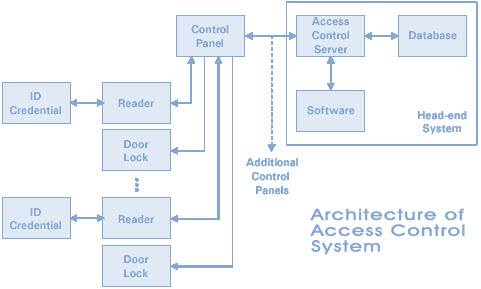
\includegraphics[width=80mm]{Architetcture-of-Access-Control-System}
    \caption{Příklad architektury přístupového systému \cite{accessControlSystem_eiprocus}}
    \label{fig:Access control system architecture}
\end{figure}

Obrázek \ref{fig:Access control system architecture} zobrazuje typickou architekturu přístupového systému, kde ID Credential představuje prvek ůmožňující identifikovat uživatele.

the user identificaton, provided for instance by RFID tag, fingerprint, QR code.
The Reader reads the data from the ID Credential and sends it to the Control Panel.
The Door Lock is used to control the physical access of users to the restricted area, e.g., building, room, floor.
The Control Panel is the interface between Access Control Server and pairs the Reader with the Door Lock. It typically connects these pairs via RS485 and Access Control Server via Ethernet, i.e., TCP/IP protocol. The main function is the management of these pairs.
The Database contains user IDs.
The Access Control Server uses Software (SW) to manage the Database and communicates with all Control Panels.
The Reader scans data from submitted ID Credential and transmits the data to the Control Panel, which resends it to the Access Control Server.
The Access Control Software finds the received user data in the Database and, if found, sends a command to the corresponding Control Panel to switch the corresponding Door Lock.
